%% Royal Society Interface manuscript
%% Built on the rsproca_new (openacc) template.

\documentclass[openacc]{rsproca_new}%%%%where rsproca is the template name

%Add here your packages or commands
\usepackage{multicol}
\usepackage[utf8]{inputenc}
\usepackage{eurosym}
\usepackage{newunicodechar}
\newunicodechar{€}{\euro{}}
\usepackage{booktabs}
\usepackage{multirow}

\addbibresource{refs.bib}

%%%% *** Do not adjust lengths that control margins, column widths, etc. ***

%%%%%%%%%%% Defining Enunciations  %%%%%%%%%%%
\newtheorem{theorem}{\bf Theorem}[section]
\newtheorem{condition}{\bf Condition}[section]
\newtheorem{corollary}{\bf Corollary}[section]
%%%%%%%%%%%%%%%%%%%%%%%%%%%%%%%%%%%%%%%%%%%%%%%

\jname{rsif}
\Journal{J R Soc Interface\ }

\begin{document}

%%%% Article title to be placed here
\title{Scaffolding without preferences: open-weight language-model agents fail the diagnostic comparative statics of two landmark social-dilemma experiments}

\author{%%%% Author details -- TODO: replace with real names/affiliations
Author 1$^{1}$}

%%%%%%%%% Insert author address here
\address{$^{1}$Affiliation, City, Country}

%%%% Subject entries to be placed here %%%%
\subject{computational social science, artificial intelligence, behavioural science}

%%%% Keyword entries to be placed here %%%%
\keywords{large language models, multi-agent simulation, social dilemmas, collective-risk dilemma, costly punishment, human surrogates}

%%%% Insert corresponding author and its email address}
\corres{Corresponding author\\
\email{tcnguyen2365@gmail.com}}

%%%% Abstract text to be placed here %%%%%%%%%%%%
\begin{abstract}

Large language model (LLM) agents are increasingly proposed as inexpensive stand-ins for human participants in social-dilemma experiments, yet whether they reproduce the social preferences that make such experiments informative remains untested. Using the FAIRGAME multi-agent framework, we replicate two landmark human studies---Milinski's collective-risk social dilemma (CRSD) and Herrmann's public-goods game (PGG) with costly peer punishment---with three open instruction-tuned models (Qwen2.5-7B, Gemma-2-9B, Llama-3.1-8B) crossed with five languages, four dispositions and sixteen societies. The models reproduce the qualitative scaffolding of cooperation but violate the diagnostic comparative statics. In CRSD they reach the climate target on 100\% of games at every loss probability (humans 50/10/0\%) and never show the human decline (\euro118$\rightarrow$\euro92$\rightarrow$\euro73) as catastrophe risk falls. In PGG, punishment does not raise contributions (P$-$N $\approx$ $-$0.36/$-$3.55/$+$0.08 tokens vs.\ human $+$4.3), and the cross-societal antisocial-punishment signature collapses (Spearman $\rho \approx -0.15$ vs.\ human $-0.90$). Current open LLMs behave like a single high-prosociality, risk-insensitive, prompt-steerable ``average cooperator''; they mimic human moves without the underlying preference structure, and are therefore not yet drop-in human surrogates where the manipulation, not the mean, carries the scientific payload.

\end{abstract}
%%%%%%%%%%%%%%%%%%%%%%%%%%%

%%%%%%%%%% Insert the texts which can accomdate on firstpage in the tag "fmtext" %%%%%

\begin{fmtext}

Can a language model stand in for a human subject? As large language models are enlisted to populate simulated societies and pre-test behavioural experiments \cite{park2023generative,argyle2023out,horton2023llm}, the appeal is obvious: agents are cheap, fast and endlessly reconfigurable. But a model that plays a cooperation game is not thereby a model that has human social preferences. The two are easy to conflate, because surface behaviour---contributing to a public good, punishing a free-rider---can look right while the latent decision structure is wrong. The decisive test is not whether agents cooperate on average, but whether they respond to the experimental \emph{manipulations} that reveal human preferences: a rising risk of catastrophe, the introduction of a punishment institution, the cross-cultural variation in punishment norms. We put three open-weight models to exactly this test, replicating two landmark human social-dilemma studies and asking where the imitation breaks down.

\end{fmtext}

%%%%%%%%%%%%%%% End of first page %%%%%%%%%%%%%%%%%%%%%

\maketitle

\begin{multicols}{2}

\section{Introduction}

Social dilemmas, in which individually rational choices aggregate into collectively irrational outcomes, are among the most consequential problems in the social and behavioural sciences \cite{dawes1980social}. From the overexploitation of a shared resource \cite{hardin1968tragedy} to the under-provision of public goods \cite{ledyard1995public}, their logic structures challenges ranging from local commons management \cite{ostrom1990governing} to the global coordination required to avert dangerous climate change. Two experimental paradigms have become canonical probes of how humans navigate these tensions. The collective-risk social dilemma (CRSD) of \cite{milinski2008climate} casts climate protection as a group investment that must reach a shared target or risk a catastrophic loss, revealing that the probability of catastrophe sharply governs how much people invest. The public-goods game with costly peer punishment of \cite{fehr2002altruistic}, scaled across societies by \cite{herrmann2008antisocial}, shows that the option to punish free-riders can sustain cooperation, but that punishment norms---including the surprising tendency to punish high contributors---vary dramatically across cultures. In each case the scientific payload lies not in the average level of cooperation but in how behaviour responds to the experimental manipulation: the risk gradient, the punishment institution, the cross-cultural contrast.

In parallel, large language models (LLMs) have rapidly emerged as candidate stand-ins for human participants in social-science research. A growing literature proposes using them as a ``silicon sample''---populations of simulated subjects whose responses can be elicited cheaply, at scale, and under conditions that would be impractical or unethical with people \cite{argyle2023out,horton2023llm}. Generative agents have been shown to produce believable individual and collective behaviour \cite{park2023generative}, to reproduce findings from classic psychology experiments \cite{aher2023using}, and to play repeated economic games with one another in ways that superficially resemble human strategic interaction \cite{akata2023playing}. This promise has motivated a broader programme asking whether LLMs can serve as behavioural models of humans at all, and whether their outputs pass a ``Turing test'' for economic and social behaviour \cite{mei2024turing}. If they do, the methodological gains for experimental social science would be substantial.

Yet playing a game competently is not the same as possessing the human preference structure that the game was designed to expose. An agent can contribute, punish, and respond to history in plausible ways while still failing to reproduce the comparative statics---the systematic shifts in behaviour across conditions---that make an experiment diagnostic of underlying preferences. Prior LLM-game research has, for the most part, examined two-player matrix games or a single model interrogated in a single language \cite{akata2023playing,brookins2023playing}, and LLMs are known to be sensitive to prompt framing and to exhibit response patterns that diverge from human distributions \cite{tjuatja2024llms}. What remains largely untested is whether these agents reproduce the diagnostic manipulations of canonical multi-player human experiments---and whether any such reproduction is robust across models, languages, and elicited dispositions, rather than an artefact of one configuration. Behavioural validity, in this setting, must be evaluated against the manipulation, not the mean.

We address this gap through two faithful replications of landmark human studies, implemented on the FAIRGAME multi-agent framework \cite{fairgame2025}. Study~1 replicates the CRSD of \cite{milinski2008climate}, preserving its six-player structure, climate cover story, fixed-target investment dynamics, hidden cumulative total, and the loss-probability treatments (90\%, 50\%, 10\%) that drive the human result. Study~2 replicates the punishment public-goods game of \cite{herrmann2008antisocial}, preserving its four-player partner matching, marginal-per-capita return, contribution-only (N) versus contribution-plus-punishment (P) treatments, and per-period relabelling. In each replication, agents read the game, its history, and a disposition or society block, reason briefly, and emit a parseable decision in lockstep simultaneous play. We cross three open instruction-tuned models---Qwen2.5-7B-Instruct \cite{qwen2025}, Gemma-2-9B-it \cite{gemma2024}, and Llama-3.1-8B-Instruct \cite{llama2024}---with five languages and four dispositional prompts, and (in Study~2) with sixteen neutral society personas drawn from the original participant cities, allowing us to test reproduction and robustness simultaneously.

Our central finding is that today's open-weight LLMs reproduce the qualitative scaffolding of human cooperation but systematically violate its diagnostic comparative statics, and we document this through three divergences. First, in the CRSD all three models reach the climate target on 100\% of games at every risk level---where humans succeeded on only 50\%, 10\%, and 0\% of groups---and pour in far more than people do, with final group totals of roughly €158--187 against human means of €118, €92, and €73; crucially, the human decline as catastrophe risk falls is absent, so the models are effectively blind to the loss-probability manipulation. Second, in the punishment game the punishment institution fails to raise cooperation and for one model significantly lowers it (treatment differences P$-$N of $-$0.36, $-$3.55, and $+$0.08 tokens, against a human grand-mean of $+$4.3), even though the models do contribute and do punish. Third, although antisocial punishment is abundant---54--59\% of all punishment points, rivalling the worst human pools---the cross-societal signature that makes Herrmann's study famous does not emerge: the human antisocial-versus-cooperation rank correlation of about $-$0.90 is absent ($-$0.15, $-$0.09, $+$0.30 across models), and the sixteen societies collapse into a contribution band roughly one token wide.

Taken together, these results indicate that current open LLMs behave like a single high-prosociality, risk-insensitive, prompt-steerable ``average cooperator'': their behavioural surface mimics human moves, but the preference structure that makes social-dilemma experiments informative---risk sensitivity, institutionally responsive conditional cooperation, and culturally heterogeneous punishment norms---is missing, even as disposition prompting shows that this behaviour is a controllable knob rather than a fixed trait. The remainder of the paper proceeds as follows. We first detail the agent protocol and the two replication designs, then report Study~1 (CRSD) and Study~2 (punishment public-goods game) in turn, before synthesising both into our central thesis and discussing its limitations and implications. We take behavioural validity here to require more than producing human-like average actions: it demands reproducing the direction and structure of behavioural change across the experimental manipulations---the risk gradient, the punishment effect, and the cross-cultural contrast---that are the very reason these experiments are informative about human social preferences.

\section{Methods}

\subsection{The collective-risk social dilemma (Study 1)}
We replicate the collective-risk social dilemma (CRSD) of \textcite{milinski2008climate}. Six players each receive a private endowment of €40 and play ten rounds. In every round each player simultaneously and privately invests €0, €2 or €4 into a shared climate account; the climate cover story matches the original. The group must accumulate a cumulative target of €120 across all players and rounds. If the target is reached, each player keeps €40 minus their own total investment; if it is missed, a single group-level lottery is drawn in which, with loss probability $p$, every player loses everything (final payoff €0), and otherwise each keeps their remainder. The catastrophe risk $p$ is crossed at three levels, $p\in\{90\%,50\%,10\%\}$, which constitutes the diagnostic manipulation of the design. There is no communication. Faithful to the original ``took notes by hand'' visibility, players observe one another's per-round contributions under fixed anonymous identifiers but are never shown the running cumulative total; the maximum attainable group total is $6\times10\times€4=€240$, twice the target. We run ten independent groups per cell.

\subsection{The public-goods game with punishment (Study 2)}
We replicate the public-goods game with costly peer punishment of \textcite{herrmann2008antisocial}. Four players are matched as partners for the whole game and play ten periods. Each period every player receives a fresh endowment of 20 tokens and contributes an integer amount between 0 and 20 to a group project with a marginal per-capita return of 0.4, so that each contributed token returns 0.4 tokens to all four members. In treatment~N players only contribute. In treatment~P the contribution stage is followed by a costly punishment stage in which each player may assign 0--10 deduction points to each other member; every point costs the punisher one token and removes three tokens from the target, the canonical 1:3 cost ratio. To block cross-period identity tracking, the other members are re-labelled every period. There is no communication, and we again run ten independent groups per cell. Following \textcite{herrmann2008antisocial}, we classify punishment by the contribution deviation between target and punisher: punishment of a target who contributed equal to or more than the punisher (deviation $\geq 0$) is \emph{antisocial}, whereas punishment of a lower contributor (deviation $<0$) is punishment of free-riding.

\subsection{Agents, models and protocol}
Each agent is an instruction-tuned LLM that receives a single natural-language prompt comprising a brief of the game rules, the history of play so far, and a disposition or society block, after which it reasons briefly and emits a parseable decision line---\texttt{CONTRIBUTION = X} in CRSD or \texttt{DEDUCT: A=a B=b C=c} in the PGG punishment stage. Within each round, all agents' decisions are collected in a single lockstep batch so that play is genuinely simultaneous. The protocol is built on the FAIRGAME multi-agent framework \parencite{fairgame2025}. We serve three open-weight instruction-tuned models, Qwen2.5-7B-Instruct \parencite{qwen2025}, Gemma-2-9B-it \parencite{gemma2024} and Llama-3.1-8B-Instruct \parencite{llama2024}, via vLLM at temperature 0.8 with fixed seeds (20080219 for CRSD, 20080307 for the PGG) to make runs reproducible; all simulations were executed offline on a single RTX PRO 6000. Each game is crossed with five languages (English, French, Arabic, Chinese, Vietnamese) and four dispositional prompts (neutral, cooperative, selfish, risk-averse); for Study~2 we additionally cross sixteen society personas drawn from the participant cities of \textcite{herrmann2008antisocial} (Boston, Copenhagen, Zurich, St.\,Gallen, Nottingham, Bonn, Seoul, Melbourne, Chengdu, Minsk, Samara, Dnipropetrovsk, Muscat, Istanbul, Riyadh and Athens), each rendered as a neutral ``You are a participant from <City>, <Country>.'' persona that carries no behavioural stereotype.

\subsection{Measures and analysis}
For Study~1 the outcome measures are target success (whether the €120 target was reached), the final group total, and the number of ``fair-sharers'' per group, defined as players whose total contribution is at least €2 per round (i.e.\ $\geq€20$). For Study~2 we measure mean per-period contribution, the antisocial share (antisocial deduction points divided by all deduction points), and deviation-binned punishment, with the punishment-institution effect summarised as the contribution difference P$-$N. We test the CRSD risk manipulation, the central diagnostic, with a one-way ANOVA of final group total across the three loss-probability treatments, computed separately per model and benchmarked against the human ANOVA ($F=13.78$, $P<0.0001$); model success rates are compared with the human baseline using Fisher's exact test and group totals using Welch's $t$-test. For the PGG, we compare treatments P and N with the Mann--Whitney $U$ test. The cross-societal signature of \textcite{herrmann2008antisocial} is assessed with the Spearman rank correlation between per-society antisocial punishment and mean contribution, and the alignment of the model's geography of cooperation with the human ordering across the sixteen societies is evaluated with Spearman rank correlations and Wilcoxon signed-rank tests. Throughout, we log the \texttt{parse\_fallback} (format non-compliance) rate for every cell and report it as a joint data-quality and fairness signal, since it varies systematically across languages. Finally, because agents in CRSD are shown per-round contributions but not the running cumulative total, any apparent target tracking must arise from the model's own arithmetic self-summation across the visible history rather than from a displayed total; we treat this arithmetic-self-summation requirement as a caveat when interpreting the models' near-uniform attainment of the target.

\section{Results}

\begin{table*}[t]
\caption{Study 1 (collective-risk climate dilemma): behaviour of the three LLM
agents in the faithful baseline (English prompt, neutral disposition, climate
framing) against the human benchmark of Milinski \textit{et al.}
\cite{milinski2008climate}, by loss probability. ``Target reached'' is the
fraction of the ten groups whose cumulative investment met the €120 threshold;
``Final total'' is the mean group investment ($\pm$ s.e.m.); ``Fair-sharers'' is
the mean number of group members (of six) investing at least €2 per round on
average. All LLM-versus-human contrasts are significant (Welch $t$ on totals and
Fisher exact on success, all $p<0.05$).}
\label{tab:crsd_baseline}
\centering
\begin{tabular}{llccc}
\toprule
Loss prob. & Player & Target reached & Final total (€) & Fair-sharers \\
\midrule
\multirow{4}{*}{90\%}
 & Human \cite{milinski2008climate} & 50\%  & 118.2 & 3.3 \\
 & Qwen2.5-7B   & 100\% & 183.0 $\pm$ 2.1 & 6.0 \\
 & Gemma-2-9B   & 100\% & 168.2 $\pm$ 3.3 & 5.8 \\
 & Llama-3.1-8B & 100\% & 177.4 $\pm$ 2.9 & 5.8 \\
\midrule
\multirow{4}{*}{50\%}
 & Human \cite{milinski2008climate} & 10\%  & 92.2  & 2.1 \\
 & Qwen2.5-7B   & 100\% & 186.6 $\pm$ 1.2 & 6.0 \\
 & Gemma-2-9B   & 100\% & 162.8 $\pm$ 2.9 & 5.9 \\
 & Llama-3.1-8B & 100\% & 165.2 $\pm$ 3.6 & 5.6 \\
\midrule
\multirow{4}{*}{10\%}
 & Human \cite{milinski2008climate} & 0\%   & 73.0  & 1.1 \\
 & Qwen2.5-7B   & 100\% & 181.0 $\pm$ 2.8 & 5.9 \\
 & Gemma-2-9B   & 100\% & 158.0 $\pm$ 3.9 & 5.8 \\
 & Llama-3.1-8B & 100\% & 170.0 $\pm$ 3.1 & 5.7 \\
\bottomrule
\end{tabular}
\end{table*}

\begin{figure*}[t]
\centering
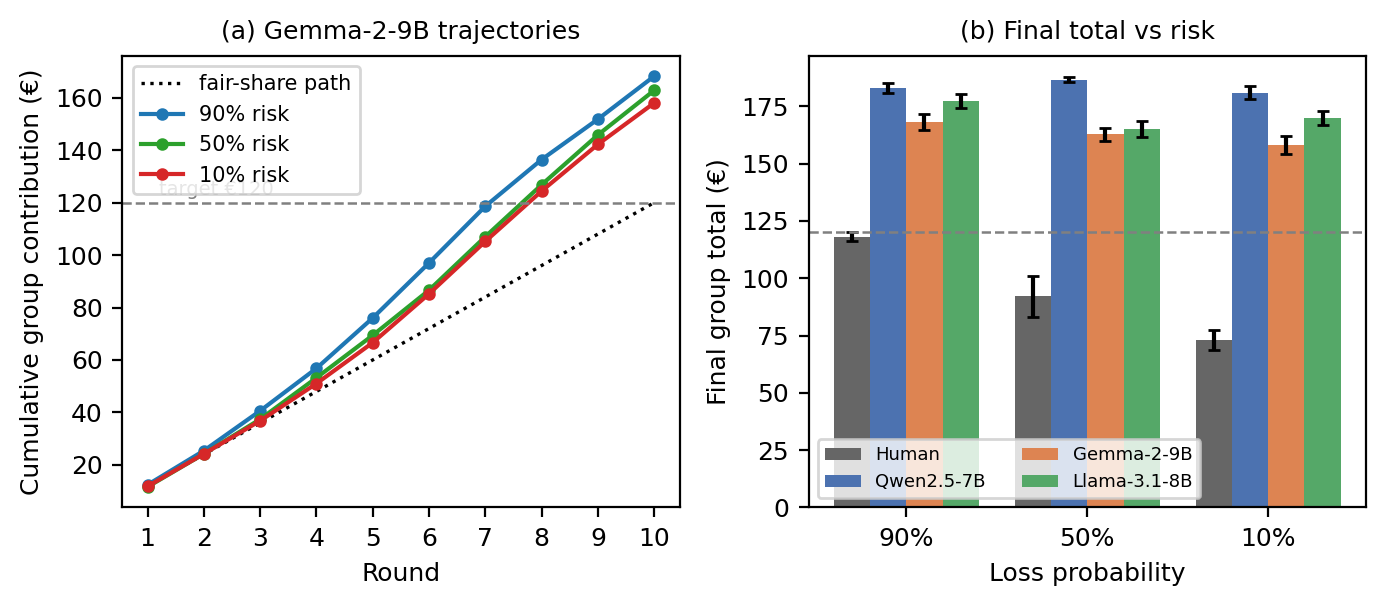
\includegraphics[width=\textwidth]{figures/fig1_crsd_risk.png}
\caption{Study 1: over-cooperation and insensitivity to catastrophe risk.
(\textit{a}) Cumulative group investment per round for Gemma-2-9B at the three
loss probabilities, against the fair-share path and the €120 target; the three
risk curves nearly coincide and all cross the target. (\textit{b}) Final group
total by loss probability for humans \cite{milinski2008climate} and the three
LLMs: humans fall steeply as catastrophe risk declines (one-way ANOVA
$F=13.78$, $p<0.0001$), whereas every model stays flat and far above target
(model ANOVA $F=1.76$/$2.23$/$3.64$). Error bars are s.e.m.}
\label{fig:crsd_risk}
\end{figure*}

\subsection{Study 1: the collective-risk climate dilemma}

In the human collective-risk dilemma, the loss probability is the lever that separates prudent from reckless groups: only half of Milinski's groups reached the €120 climate target under the gravest 90\% catastrophe risk, one in ten reached it at 50\%, and none reached it at 10\%, with final group totals falling from €118 through €92 to €73 as the threat receded \cite{milinski2008climate}. The LLM agents show no such restraint. In the English, neutral, climate-framed baseline, all three models---Qwen2.5-7B-Instruct, Gemma-2-9B-it and Llama-3.1-8B-Instruct---reach the target on 100\% of games at every loss probability (table~\ref{tab:crsd_baseline}), and they do so by over-investing rather than by tracking the threat: final group totals cluster between roughly €158 and €187, some 70--78\% of the €240 ceiling attainable if every player invested the maximum in every round, and far above the human totals of €118, €92 and €73. The same over-supply is visible in the count of ``fair-sharers'': where human groups typically contained only one to three players investing at least €20 over the game, the model groups contain roughly six of six. Welch tests on final totals and Fisher exact tests on success counts confirm that these model--human gaps are statistically significant across the board (table~\ref{tab:crsd_baseline}).

The decisive diagnostic, however, is not the level of cooperation but its insensitivity to risk. In humans the loss-probability manipulation is what drives behaviour, producing a steep and monotone decline (one-way ANOVA across the three treatments $F=13.78$, $P<0.0001$). The models reproduce none of this gradient: the analogous ANOVA on final group totals yields only $F=1.76$ ($P=0.19$) for Qwen, $F=2.23$ ($P=0.13$) for Gemma and $F=3.64$ ($P=0.040$) for Llama, and even the lone nominally significant case is weak and non-monotone rather than the orderly human descent. Figure~\ref{fig:crsd_risk}a makes the failure concrete: the cumulative-contribution trajectories for 90\%, 50\% and 10\% loss risk nearly coincide and all cross the €120 target well before the final round, regardless of how much is actually at stake. Figure~\ref{fig:crsd_risk}b sharpens the contrast by plotting final total against loss probability: the human line falls steeply as catastrophe risk recedes, whereas all three model lines stay essentially flat and far above target. The manipulation that makes the experiment informative about human risk preferences leaves the models almost untouched.

\begin{figure*}[t]
\centering
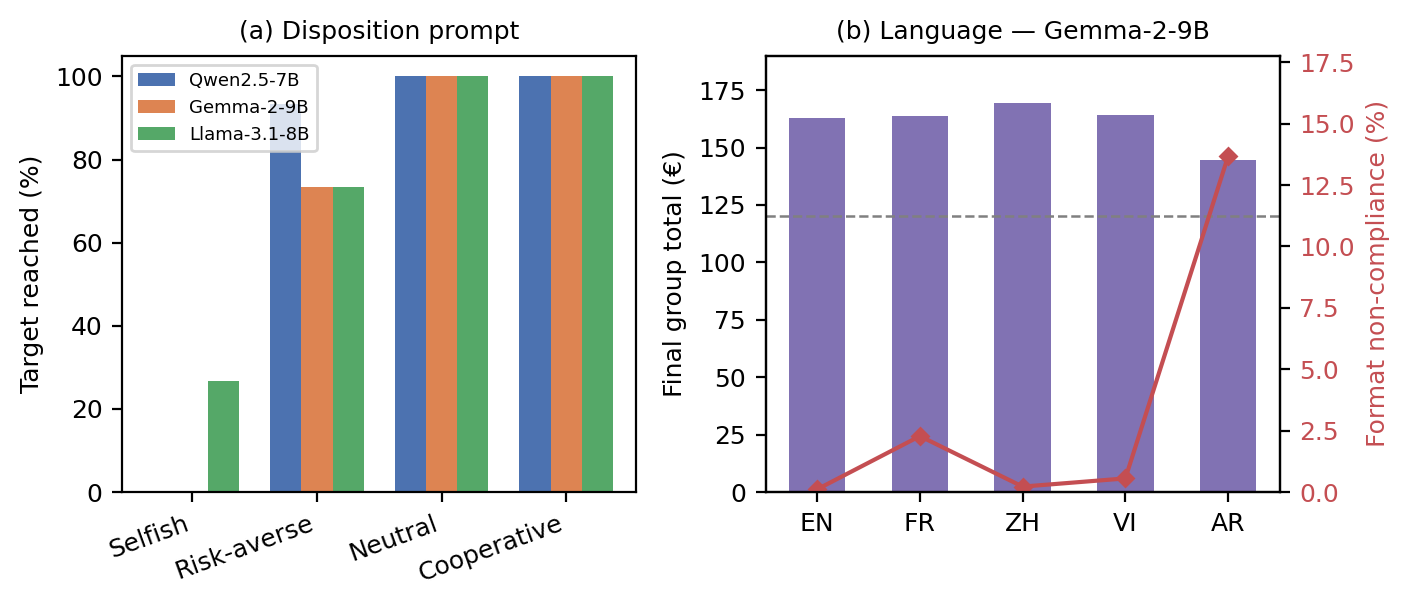
\includegraphics[width=\textwidth]{figures/fig2_crsd_moderators.png}
\caption{Study 1 moderators. (\textit{a}) Target-success rate by dispositional
prompt: a ``selfish'' instruction collapses cooperation (0\% success for Qwen
and Gemma), ``risk-averse'' is intermediate, and ``neutral''/``cooperative''
sit at the ceiling, showing that the default high-prosociality behaviour is a
steerable knob. (\textit{b}) Gemma-2-9B final total (bars) and format
non-compliance rate (line) by prompt language: cooperation is broadly
language-invariant in content, but format reliability degrades sharply in
Arabic.}
\label{fig:crsd_moderators}
\end{figure*}

That the default behaviour is a high-prosociality persona rather than a fixed trait becomes clear once disposition is varied. The dispositional prompt is a powerful lever on the same models (figure~\ref{fig:crsd_moderators}a): switching the agents from neutral to a selfish disposition collapses target success from the ceiling to 0\% for Qwen and Gemma and to 27\% for Llama, with final group totals dropping into the €33--113 range and many groups now missing the target outright. A risk-averse disposition produces an intermediate regime (success between 73\% and 93\%), while the neutral and cooperative prompts both sit at or near the 100\% ceiling. The behaviour therefore moves across almost the entire feasible range under prompt control, which indicates that the over-cooperative baseline reflects a steerable default persona rather than an immovable property of the architecture---a knob, not a trait.

Finally, the core result is robust across languages while exposing a low-resource fragility that is a fairness caveat rather than an explanation. Translating the game into French, Chinese, Vietnamese and Arabic leaves the substantive outcomes roughly invariant: the models still over-cooperate and still ignore the risk gradient. What does vary is format compliance. The rate of format non-compliance (parse-fallback) stays below 2.5\% in most cells but spikes to 13.7\% for Gemma in Arabic and 14.8\% for Llama in Vietnamese (figure~\ref{fig:crsd_moderators}b), a non-trivial degradation that the framework logs as a data-quality and fairness signal. Crucially, the English baseline that carries the over-cooperation result has a parse-fallback rate of essentially 0\%, so the failure to track risk cannot be dismissed as an arithmetic or parsing artefact: the models read the game correctly and still pour in resources regardless of the odds.

\begin{table*}[t]
\caption{Study 2 (public goods with peer punishment): mean contribution (of 20
tokens) in the faithful baseline (English prompt, neutral disposition) without
(N) and with (P) a punishment stage, the punishment effect $\Delta=\bar c_P-\bar
c_N$, and the antisocial share of all punishment (points aimed at members who
contributed equal to or more than the punisher). The human reference is the
16-pool grand mean of Herrmann \textit{et al.}\ \cite{herrmann2008antisocial},
where punishment raised cooperation ($\Delta\approx+4.3$) and antisocial
punishment, though present, was a minority of expenditure in most pools.
$p$ from a two-sided Mann--Whitney $U$ test on the ten per-group means
(P vs N).}
\label{tab:pgg_baseline}
\centering
\begin{tabular}{lccccc}
\toprule
Player & Contrib.\ N & Contrib.\ P & $\Delta$ (P$-$N) & $p$ & Antisocial share \\
\midrule
Human \cite{herrmann2008antisocial} & 8.6 & 12.9 & $+4.3$ & --- & minority\textsuperscript{*} \\
Qwen2.5-7B   & $14.26 \pm 0.48$ & $13.90 \pm 0.51$ & $-0.36$ & 0.71   & 59\% \\
Gemma-2-9B   & $13.41 \pm 0.37$ & $9.86  \pm 0.37$ & $-3.55$ & $<$0.001 & 55\% \\
Llama-3.1-8B & $10.67 \pm 0.45$ & $10.75 \pm 0.43$ & $+0.08$ & 0.91   & 54\% \\
\bottomrule
\end{tabular}
\\[2pt]
{\footnotesize \textsuperscript{*}In Herrmann \textit{et al.}\ the antisocial
share varied widely across societies but prosocial punishment of free-riding
dominated in most Western pools.}
\end{table*}

\begin{figure*}[t]
\centering
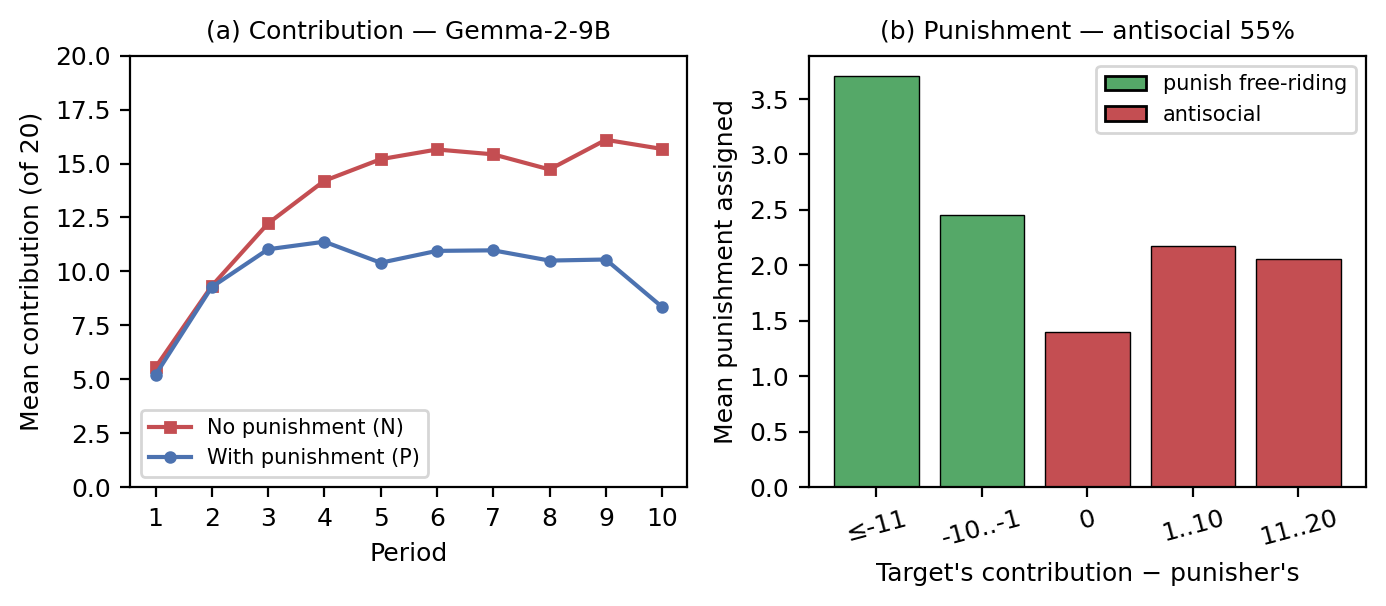
\includegraphics[width=\textwidth]{figures/fig3_pgg_punishment.png}
\caption{Study 2: punishment dynamics for Gemma-2-9B. (\textit{a}) Mean
contribution per period without (N) and with (P) punishment: the punishment
treatment lies \textit{below} the no-punishment baseline, the opposite of the
human result that punishment sustains cooperation. (\textit{b}) Mean punishment
assigned by the contribution deviation of the target relative to the punisher;
green bars are prosocial punishment of free-riding, red bars are antisocial
punishment of equal or higher contributors, which accounts for 55\% of all
expenditure.}
\label{fig:pgg_punishment}
\end{figure*}

\subsection{Study 2: public goods with peer punishment}
\label{sec:results_pgg}

In the contribution-only treatment (N) all three models sustained substantial cooperation, with baseline mean contributions of $14.26\pm0.48$ (Qwen), $13.41\pm0.37$ (Gemma) and $10.67\pm0.45$ (Llama) tokens of the 20-token endowment (table~\ref{tab:pgg_baseline})---comfortably above the human grand-mean of $8.6$ tokens \cite{herrmann2008antisocial}. The diagnostic test, however, is whether adding a costly peer-punishment stage (treatment P) lifts cooperation, the central result of the punishment literature \cite{fehr2002altruistic,herrmann2008antisocial}. It does not. The within-model difference $\mathrm{P}-\mathrm{N}$ was $-0.36$ tokens for Qwen, $-3.55$ for Gemma and $+0.08$ for Llama, against a human grand-mean gain of approximately $+4.3$ tokens (from $8.6$ under N to $12.9$ under P). For two of the three models the punishment institution thus left cooperation flat or, in Gemma's case, drove it significantly \emph{down} (Mann--Whitney $p<0.001$; the per-period $\mathrm{N}>\mathrm{P}$ trajectory is shown in figure~\ref{fig:pgg_punishment}a), while for Qwen the small decline was not significant ($p=0.71$) and Llama's near-zero change likewise did not differ from chance ($p=0.91$). The institutional responsiveness that makes punishment informative about human conditional cooperation is therefore absent.

The punishment that the models did assign, moreover, was substantially antisocial. Classifying each deduction by the contribution deviation between target and punisher, antisocial punishment---points aimed at a target who contributed equal to or more than the punisher (deviation $\geq 0$)---accounted for $59\%$, $55\%$ and $54\%$ of all points for Qwen, Gemma and Llama respectively, rivalling the most punitive human participant pools \cite{herrmann2008antisocial}. Yet the deviation-binned structure of that punishment (figure~\ref{fig:pgg_punishment}b) reveals that the models differ sharply in whether they retain the human-like logic of punishing deeper free-riding more harshly. Only Gemma reproduced the monotone gradient, escalating from $2.45$ points in the mild-free-riding bin to $3.71$ points for the most extreme free-riders (deviation $\leq -11$) while sparing equal contributors ($1.40$ points at deviation $0$). Qwen and Llama, by contrast, punished almost uniformly across deviation bins, meting out comparable deductions to free-riders and cooperators alike: Qwen ranged only from $2.15$ to $2.78$ points and Llama from $2.53$ to $2.86$ points across the full deviation spectrum, punishing equal-or-higher contributors ($2.29$ and $2.60$ points at deviation $0$) nearly as hard as the worst free-riders. The behavioural surface of punishment is present, but for two models the underlying targeting logic that distinguishes prosocial from antisocial sanctioning is not.

\begin{figure*}[t]
\centering
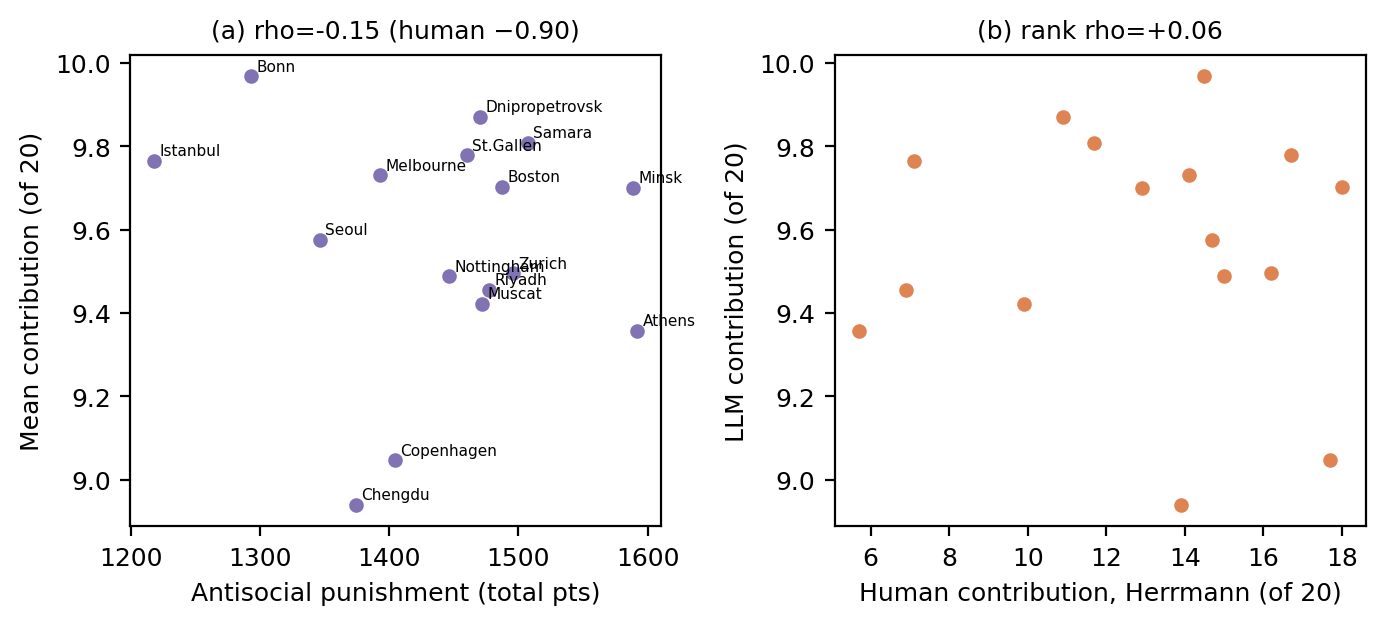
\includegraphics[width=\textwidth]{figures/fig4_pgg_cross_societal.png}
\caption{Study 2: the cross-societal signature is not reproduced.
(\textit{a}) Per-society antisocial punishment versus mean contribution for the
16 city personas (Gemma-2-9B): the strong negative association seen in humans
(Spearman $\rho\approx-0.90$) is absent ($\rho=-0.15$). (\textit{b}) LLM versus
human \cite{herrmann2008antisocial} mean contribution across the same societies:
the model compresses every society into a $\sim$1-token band and does not
reproduce the human ranking (rank $\rho=+0.06$).}
\label{fig:pgg_cross}
\end{figure*}

Most consequentially, the cross-societal signature that makes Herrmann's study diagnostic of culturally heterogeneous norms fails to emerge. In the human data, pools where antisocial punishment is prevalent are those where cooperation is low, yielding a strong negative rank correlation of approximately $-0.90$ between per-society antisocial punishment and mean contribution \cite{herrmann2008antisocial}. Across our sixteen neutral city personas this relationship was effectively flat: the antisocial-versus-cooperation Spearman correlation was $-0.09$ for Qwen, $-0.15$ for Gemma and $+0.30$ for Llama (figure~\ref{fig:pgg_cross}a)---in Llama's case of the opposite sign. The accompanying ``geography of cooperation'' also collapsed: society personas shifted contribution by only about one token, compressing all sixteen cities into a narrow band rather than reproducing the broad human cross-cultural spread (figure~\ref{fig:pgg_cross}b). The models did not even rank the societies as humans do, with LLM-versus-human cross-societal rank correlations of just $+0.33$ (Qwen), $+0.06$ (Gemma) and $+0.17$ (Llama), and the overall level of cooperation differed from the human pools for two of the three models (Wilcoxon $p=0.005$ for Gemma and $p=0.025$ for Llama, mean LLM$-$human differences of $-3.30$ and $-2.47$ tokens; Qwen did not differ, $p=0.67$). Thus, even where the models do punish, contribute and engage in antisocial sanctioning, the culturally structured preference heterogeneity that is the scientific payload of the original experiment is missing.

\section{Discussion}

Across two landmark social dilemmas, replicated faithfully on the FAIRGAME framework \cite{fairgame2025} with three open instruction-tuned models, the same pattern emerges twice. The qualitative scaffolding of human cooperation is present: agents contribute to the shared climate account and reach the target in the collective-risk dilemma (Study~1), they contribute to the group project and assign costly punishment to others in the public-goods game (Study~2), they engage in antisocial as well as pro-social punishment, and their behaviour bends predictably to a dispositional prompt. Read at the level of moves made, the models look like cooperators in a cooperation experiment. Yet the diagnostic comparative statics---the responses to the experimental \emph{manipulations} that are precisely what make these designs informative about human social preferences \cite{milinski2008climate, herrmann2008antisocial}---do not reproduce. In Study~1 the loss-probability gradient that drives human behaviour is effectively flat (figure~\ref{fig:crsd_risk}): humans pour in steadily less as catastrophe becomes less likely, whereas all three models reach the target on every game at every risk level and sit far above the human totals, indifferent to the very variable the experiment manipulates. In Study~2 the punishment institution that lifts cooperation in human pools fails to do so, and for one model significantly depresses it (figure~\ref{fig:pgg_punishment}), while the cross-societal signature that made the original study famous---the strong negative coupling between antisocial punishment and cooperation, and the heterogeneity across cities---collapses into a near-zero correlation and a contribution band barely a token wide (figure~\ref{fig:pgg_cross}). The two studies therefore converge on a single conclusion: surface cooperation survives, but the structure underneath it does not.

The most parsimonious reading, which we offer as a behavioural characterisation rather than a claim about model internals, is that the current generation of open-weight models behaves like a single high-prosociality, risk-insensitive, prompt-steerable ``average cooperator''. Three properties define this profile. It is \emph{high-prosociality}: contributions cluster well above human means and at or near the cooperative ceiling, and the punishment that is deployed is as often antisocial as corrective. It is \emph{risk-insensitive} and, more broadly, insensitive to institutional and cultural structure: the loss-probability gradient, the punishment-institution effect, and the geography of cooperation across societies are all attenuated or absent, so the manipulations that carry the scientific payload in human work leave the model essentially unmoved. And it is \emph{prompt-steerable}: the dispositional prompt is a genuine and large lever---a selfish framing collapses target success while cooperative and neutral framings hold near the ceiling (figure~\ref{fig:crsd_moderators})---which shows that the prosocial set point is a controllable knob rather than a fixed trait, but a knob the experimenter sets explicitly rather than a preference the agent brings to the table. What is missing is exactly the thing these experiments were built to measure: a human-like preference structure in which cooperation is conditional, responsive to incentives and institutions, sensitive to risk, and heterogeneous across populations. The models reproduce the behavioural surface while lacking that underlying structure---a thin behavioural layer that mimics human moves without the generative machinery that produces them.

These findings bear directly on the growing programme that treats LLMs as ``silicon subjects'' or simulated participants for social science \cite{argyle2023out, horton2023llm, park2023generative}. That programme rests on an implicit assumption: that a model which produces human-like responses on average also responds to interventions the way humans do, so that one can run a manipulation \emph{in silico} and read off the treatment effect. Our results sharpen where that assumption holds and where it breaks. For descriptive or generative purposes---populating an environment with plausible cooperators, stress-testing an interface, prototyping a design before a costly human study---the qualitative scaffolding is real and usable. But for the inferential purpose that motivates most of this literature, namely estimating how behaviour shifts when an experimenter varies risk, institutions, or cultural context, the models are not yet drop-in surrogates: the mean is reproduced but the manipulation is not, and it is the response to the manipulation, not the mean, that constitutes the validity test. This is consistent with a wider scepticism about whether LLMs reproduce the distributional and conditional structure of human responses rather than a central-tendency caricature \cite{mei2024turing, tjuatja2024llms}. The practical recommendation is to validate the comparative statics, not merely the marginal behaviour, before substituting an agent for a subject.

The results also carry implications for deploying LLM agents in genuinely multi-agent, cooperative settings rather than as proxies for people. A population of homogeneous, highly prosocial, risk-insensitive agents has appealing properties---it cooperates readily and resists collapse into mutual defection---but it is also fragile in instructive ways. Its prosociality is not robustly conditional: punishment institutions that discipline free-riders in human groups do not reliably steer these agents, and a large fraction of the punishment that is issued is antisocial, directed at equal-or-higher contributors. An agent collective that cannot use sanctioning institutions to stabilise cooperation, and that turns punishment against good citizens, will behave unpredictably once incentives, adversarial participants, or heterogeneous objectives enter the picture. At the same time, the strong dispositional steerability we document is a design affordance: because the prosocial set point is a controllable knob, system designers can dial cooperative behaviour up or down by prompt, which is useful for orchestration but also a reminder that the resulting cooperation is imposed from outside rather than emergent from the agents' own incentives. Both observations counsel caution about assuming that multi-agent LLM systems will spontaneously reproduce the institutional and normative mechanisms that sustain human cooperation.

\subsection{Limitations}

Several limitations qualify these conclusions and bound their scope. First, we study three open-weight models in the 7--9B parameter range at a single sampling temperature; we make no claim about frontier or proprietary systems, larger open models, or other decoding regimes, any of which might exhibit a richer preference structure. The ``average cooperator'' characterisation is a statement about this accessible, reproducible class of models, not about LLMs in general. Second, the collective-risk design carries a self-summation confound: faithful to the original, agents are shown each player's per-round contributions but not the running cumulative total, so reaching the €120 target requires the agent to track and add contributions across rounds, and apparent over-cooperation could in principle reflect arithmetic difficulty rather than a behavioural choice. We mitigate this concern---the English baseline parse-fail rate is essentially zero (figure~\ref{fig:crsd_moderators}), so the decisions are well-formed and the over-cooperation is not a parsing artefact---but we cannot fully exclude that imperfect mental accounting contributes to the flat risk response, and we flag it candidly.

Third, format non-compliance is itself double-edged. In most conditions parse-fallback is below a few per cent, but it rises sharply in particular language-model pairings (notably Gemma in Arabic and Llama in Vietnamese), where a non-trivial fraction of decisions are not emitted in parseable form. This is at once a confound, because excluded or fallback decisions can bias the surviving sample, and a substantive fairness signal, because it shows that behavioural and even basic instruction-following capability is unevenly distributed across languages---a finding worth reporting in its own right rather than merely cleaning away. Fourth, our society personas are deliberately neutral, of the form ``you are a participant from \textless city\textgreater'', with no behavioural stereotype attached. This is a principled choice that avoids injecting the experimenter's own cultural priors, but it may under-elicit the cultural variation the cross-societal analysis seeks: the geography of cooperation could be thicker under richer, more contextualised personas, and our null result speaks to neutral city labels specifically rather than to cultural conditioning in general.

Fifth, our games are single-shot in the sense that agents play with no fine-tuning, no learning across episodes, and no communication between players, under prompts to which behaviour is demonstrably sensitive. We have shown that disposition prompting moves behaviour substantially, which is a strength for controllability but also means that point estimates depend on prompt design choices; we have not exhaustively mapped that sensitivity. Finally, and cutting across all of the above, the instruction-tuning and alignment processes that make these models usable are themselves likely to inflate prosociality, pushing the agents toward helpful, agreeable, conflict-averse behaviour. This offers a plausible partial account of both the high cooperative set point and the muted responsiveness to risk and sanction, but it is a conjecture about training rather than a measured cause, and we do not claim to have isolated it.

These limitations chart the natural next steps. The clearest is to extend the same faithful protocol to larger and frontier models, to test whether scale or additional capability restores any of the missing comparative statics. Beyond scale, richer and more strongly contextualised personas would test whether cultural heterogeneity can be elicited at all; adding inter-agent communication would let conditional cooperation and reciprocity emerge dynamically rather than being read from one-shot decisions; and training agents with reinforcement learning in these environments, rather than relying on instruction-tuned priors, would test whether a genuine, incentive-grounded preference structure can be induced where the current thin behavioural surface falls short.

\section{Conclusion}

We replicated two diagnostic human social-dilemma experiments---the collective-risk climate dilemma and the public-goods game with costly peer punishment---with three open-weight LLM agents crossed with languages, dispositions, and societies, and asked whether today's open models are behaviourally valid stand-ins for human subjects. They reproduce the qualitative scaffolding of human cooperation but systematically violate the comparative statics that make these experiments informative: they hit the climate target regardless of catastrophe risk, they are not lifted by a punishment institution, and they show none of the cross-cultural heterogeneity in punishment and cooperation that defines the human data. The behaviour is best described as a single high-prosociality, risk-insensitive, prompt-steerable average cooperator---a thin behavioural surface that mimics human moves without the human preference structure beneath them. The constructive corollary is that these agents are well suited to qualitative scaffolding and serve as a genuinely steerable behavioural testbed, but they are not yet drop-in human surrogates for studies whose scientific payload lies in a manipulation rather than a mean \cite{horton2023llm, fairgame2025}. The validity test for a silicon subject is not whether it cooperates, but whether it responds to the experiment's interventions the way a human would; on that test, the manipulation, not the mean, is what current open models still fail to reproduce.

\end{multicols}

\enlargethispage{20pt}

\ethics{This study involved no human or animal participants. All behavioural data were generated by computational simulations of large language models and therefore required no ethics approval.}

\dataccess{The simulation code, prompt templates, configuration files, per-game result files for all three models, and the analysis script (\texttt{analysis/analyze.py}) that regenerates every figure and table are available in the project repository. The human benchmarks are taken from the published data of Milinski \textit{et al.}\ \cite{milinski2008climate} and Herrmann \textit{et al.}\ \cite{herrmann2008antisocial}.}

\aucontribute{Insert author contributions text here.}

\competing{The author(s) declare that they have no competing interests.}

\funding{Insert funding text here.}

\ack{We thank the developers of the FAIRGAME framework and of the vLLM inference engine. The simulations used the Qwen2.5, Gemma~2 and Llama~3.1 open-weight models.}

\disclaimer{Large language models were used solely as the objects of study (the simulated agents); all analysis, figures and text were produced and verified by the authors.}

%%%%%%%%%% Insert bibliography here %%%%%%%%%%%%%%

\printbibliography

\end{document}
